\chapter{Probabilidades de uso}
\label{sec:learning}


%\subsection{Aprendizaje autom\'atico desde un corpus para describir nuevos objetos}

En el cap\'itulo anterior hemos presentado un algoritmo que supone que para
cada relaci\'on R se tiene una conocida probabilidad de uso R.\puse. En esta secci\'on, se dan algunas posibilidades de c\'omo
calcular estas probabilidades de uso.

Por otro lado, al ser nuestro algoritmo no-determinista en 2 ejecuciones podr\'ia dar diferentes ER para el mismo target y conjunto de probabilidades de uso, incluso si estas son aleatorias.

Luego en el Cap\'itulo \ref{sec:evaluacion} veremos como las probabilidades de uso calculadas como se muestra ac\'a nos dan una buena aproximaci\'on a la frecuencia de ocurrencia de las ER en corpus.

\section{Aleatoriamente}

Una posibilidad es dar a cada relaci\'on de la signatura del modelo, una probabilidad de uso aleatoria, es facil de calcular, y dado que el algoritmo asegura dar una expresi\'on referencial si existe, calcular las probabilidades de uso en forma aleatoria ser\'ia una posibilidad.

\section{Uniformemente}

Lo malo de poner esto aca, es que la forma en que lo evaluamos despues no fue exactamente asi, fue uniforme en las er no en las prob de uso... pensar si dejo esto...

\section{A partir de corpus}

Supongamos que tenemos disponible un corpus de ER asociada a diferentes escenas t\'{i}picas del dominio en el que el algoritmo GER tiene que operar. 


\subsection{Calculando \puse\ cuando hay disponible un corpus para la escena considerada}

Las Figuras \ref{rojo-amarillo} y  \ref{verde-azul} son las escenas del corpus GRE3D7 introducido en \ref{sec:corpusGRE}, est\'an agrupadas seg\'un los colores que tienen.\\




\begin{figure}
\centering
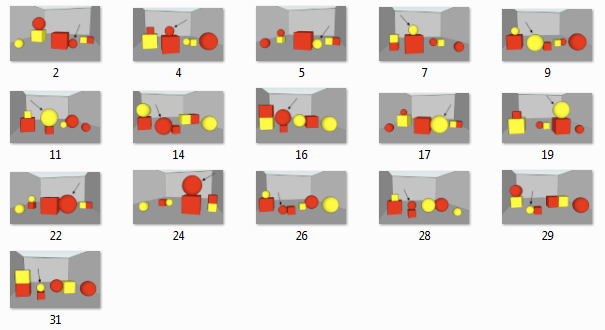
\includegraphics[width=1\textwidth]{images/rojo-amarillo.png}
\caption{Im\'agenes del GRE3D7 parte rojo y amarillo}
\label{rojo-amarillo}
\end{figure}

\begin{figure}
\centering
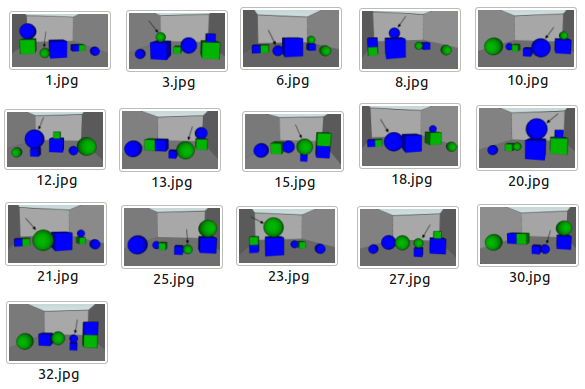
\includegraphics[width=1\textwidth]{images/imagenesML.png}
\caption{Im\'agenes del GRE3D7 parte azul y verde}
\label{verde-azul}
\end{figure}



\begin{figure}[ht]
\begin{minipage}[b]{0.5\linewidth}
\centering
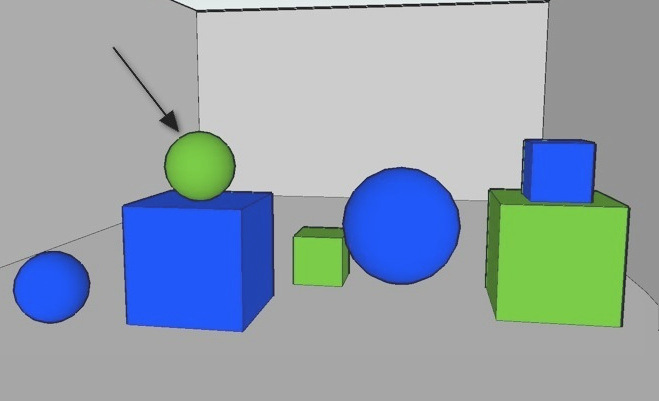
\includegraphics[width=\textwidth]{images/3.jpg}
%\vspace*{1cm}
\caption{Contexto 3 del GRE3D7}
\label{fig3}
\end{minipage}
\hspace*{1cm}
\begin{minipage}[b]{0.5\linewidth}
%\centering
%\begin{figure}[ht]
%\begin{center}
green ball \\
small green ball  \\
small green ball on-top red large cube \\
green ball on-top blue cube\\
green ball on-top large blue cube \\
small green ball on-top blue cube  \\
ball on-top cube \\
small green ball on-top red large left cube  \\
small ball on-top cube large  \\
top green ball   \\
green ball on-top cube  \\
\caption{ER dadas por personas para el Contexto \ref{fig3}}
\label{ER-fig3}
\end{minipage}
\end{figure}


El corpus tiene para cada imagen 140 ER dadas por personas. Las ER dadas en \ref{ER-fig3} son las ER diferentes que aparecieron en el corpus para el Contexto \ref{fig3}, pero... uno se imagina un corpus en que las personas usaron distintas palabras para nombrar lo mismo, distintas frases, distinto orden de las palabras, s\'i es verdad, este corpus ya est\'a limpio de todas esas cosas, pero si quisieramos partir de un corpus con las ER tal cual dieron las personas, tendr\'iamos que realizar los siguientes pasos a fin de unificar el vocabulario:

\begin{enumerate}
\item Tokenizar las expresiones referenciales y llamar al conjunto de palabras distintas
 $Pal$. En particular, las expresiones de varias palabras como ``arriba de'', ``encima de''
  debe ser igualadas a una \'unica palabra que signifique lo mismo, digamos \emph{arriba-de}.

\item Eliminar hiper\'onimos de $Pal$. Por ejemplo, si ambos \emph{cubo} y
  \emph{cosa} aparecen en $Pal$ para nombrar la misma cosa, eliminar \emph{cosa}, ya que \emph{cubo} es m\'as espec\'ifico.

\item Si el conjunto de palabras obtenidas en los pasos anteriores contiene
  sin\'onimos normalizarlos con un representante de la clase.  Por ejemplo, las palabras \emph{chico}
  y \emph{peque\~no} son ambas representadas por la palabra \emph{peque\~no}.

\item Llamar al conjunto resultante $\REL$; que ser\'a la signatura del modelo $\gM$ utilizada por el algoritmo.

\item Para cada escena, definir $\gM$ tal que la interpretaci\'on
 $\interp {\cdot}$ asegure de que todas las ERs encontradas en el corpus sean ER en
  el modelo. Por ejemplo, las %$\el$ f\'ormulas correspondientes%
	ER de \ref{ER-fig3} deben denotar el target se\~nalado en la Figura \ref{fig3} el modelo 
$\gM$ est\'a representado en Figura~\ref{modelo-fig3}.
%GRE3D7-stimulus-cap2
\item Para cada R$\in \REL$ calculo R.\puse \ utilizando~(\ref{eq1}) si
  hay muchas ER para cada escena (caso corpus GRE3D7) o asignamos 1 a R.\puse \ si R esta en ER, asignamos 0 en caso contrario (caso corpus TUNA).
\end{enumerate}

En el caso del GRE3D7 ya estaba unificado el vocabulario y la signatura del modelo es 
$\REL = \{green, ball, small, ontop, red, large, cube, blue, left, top\} $

\begin{figure}[ht]
\centering
\begin{tikzpicture}
  [
    n/.style={circle,fill,draw,inner sep=3pt,node distance=2cm},
    aArrow/.style={->, >=stealth, semithick, shorten <= 1pt, shorten >= 1pt},
  ]
 \node[n,label=above:$e_1$,label=below:{
    \relsize{-1}$\begin{array}{c}
      \nLeft\\[-2pt]
      \nSmall\\[-2pt] 
      \nBlue\\[-2pt]
      \nBall\end{array}$}] (a) {};

 \node[n,label=above:$e_2$,label=below:{
    \relsize{-1}$\begin{array}{c}
      \nLeft\\[-2pt]
      \nBig\\[-2pt] 
      \nBlue\\[-2pt]
      \nCube\end{array}$}, right of=a] (b) {};

 \node[n,label=below:$e_3$,label=above:{
    \relsize{-1}$\begin{array}{c}
      \nTop\\[-2pt]      
			\nLeft\\[-2pt]
      \nSmall\\[-2pt]      
			\nGreen\\[-2pt]
      \nBall\end{array}$}, above of=b] (c) {};

 \node[n,label=above:$e_4$,label=below:{
    \relsize{-1}$\begin{array}{c}
      \nSmall\\[-2pt] 
      \nGreen\\[-2pt] 
      \nCube\end{array}$}, right of=b] (d) {};

 \node[n,label=above:$e_5$,label=below:{
    \relsize{-1}$\begin{array}{c}
      \nBig\\[-2pt] 
      \nBlue\\[-2pt] 
      \nBall\end{array}$}, right of=d] (e) {};

 \node[n,label=above:$e_6$,label=below:{
    \relsize{-1}$\begin{array}{c}
      \nBig\\[-2pt] 
      \nGreen\\[-2pt] 
      \nCube\end{array}$}, right of=e] (f) {};

 \node[n,label=below:$e_7$,label=above:{
    \relsize{-1}$\begin{array}{c}
      \nTop\\[-2pt]
      \nSmall\\[-2pt]
      \nBlue\\[-2pt]
      \nCube\end{array}$}, above of=f] (g) {};

 \draw [aArrow,bend right=90] (b) to node[auto,swap]{\relsize{-1}$\nBelow$} (c);
 \draw [aArrow,bend right=90] (c) to node[auto,swap]{\relsize{-1}$\nOntop$} (b);

 \draw [aArrow,bend right=30] (d) to node[auto,swap]{\relsize{-1}$\nLeftof$} (e);
 \draw [aArrow,bend right=30] (e) to node[auto,swap]{\relsize{-1}$\nRightof$} (d);

 \draw [aArrow,bend right=90] (f) to node[auto,swap]{\relsize{-1}$\nBelow$} (g);
 \draw [aArrow,bend right=90] (g) to node[auto,swap]{\relsize{-1}$\nOntop$} (f);
\draw[dotted] (-0.5,-1.4) rectangle (9.7,3.7);
 %\draw[dotted] (-.65,-1.2) rectangle (7.1,2.1);

 \end{tikzpicture}
\vspace*{-.4cm}\caption{El modelo del Contexto \ref{fig3}}
\label{modelo-fig3}
\end{figure}

La regresi\'on lineal es un m\'etodo matem\'atico que modela la relaci\'on que hay entre una variable dependiente Y, las variables independientes Xi y un t\'ermino aleatorio E.  \\

Vamos a tomar la parte \ref{verde-azul} del corpus GRE3D7 para aprender las probabilidades de uso de cada palabra en las ER que di\'o la gente, y as\'i darnos una idea de como es la distribuci\'on del uso de las palabras del conjunto $REL$ en el corpus.\\

Vamos a usar las siguientes propiedades, las cuales las sacamos autom\'aticamente del XML del corpus.

\begin{small}
\begin{table}[h]
\begin{center}
\begin{tabular}{|l|p{10cm}|}
\hline
target-tiene & cuando el elemento target tiene la propiedad. \\
\#rel-prop & n\'umero de propiedades y relaciones que el target tiene.\\
\#rel & n\'umero de relaciones que el target tiene. \\
landmark-tiene & cuando un landmark del target tiene la propiedad, un objeto es un landmark si tiene una relaci\'on directa en el modelo, con el target (lo usamos para el GRE3D7).\\
location-has & cuando la RE puede usar la ubicaci\'on del target en la figura (esto se hizo porque el TUNA corpus tiene algunas ER donde se le dijo a la gente que pod\'ian usar la localizaci\'on del objeto).\\
discrimination & calculada como 1 sobre el n\'umero de objetos en el modelo que tienen la propiedad.  \\
\hline
\end{tabular}
\caption{Caracter\'isticas usadas para conseguir f\'ormulas con regresi\'on lineal que nos den una idea de la \puse\ de las palabras} 
\label{features}
\end{center}
\end{table}
\end{small}

\begin{table}[h!]
\begin{center}
\caption{F\'ormulas y errores de regresi\'on lineal para todo el corpus \ref{verde-azul}}
\label{tabla-linear-regresion-all}
\begin{tabular}{|l|c|c|l|}
\hline
Palabra &Error promedio	LR	& Error-PM	& F\'ormula de LR\\
\hline
ball		 &0.0465   &0.0609	  & 0.2894 * disc-gatt + 0.7883\\
\hline
cube		 &0.0417	 &0.0531	  &0.49   * disc-gatt - 0.0129\\
\hline
\hline
blue		 &0.0353	 &0.0454	  &0.848  * target-tiene + 0.1073\\
\hline
green		 &0.0264	 &0.046	    &0.8722 * target-tiene + 0.0016\\
\hline
\hline
large		 &0.1762	 &0.2378	  &0.5911 * target-tiene + 0.0354\\
\hline
small		 &0.1499	 &0.1755	  &0.3918 * target-tiene + 0.2478 * landmark-tiene -\\
				 &				 &					&0.0913\\
\hline
\hline
left-of  &0.0041	 &0.0094	  &0.0131 * target-tiene +\\
				 &				 &					&0.0253 * adj-target-tiene - 0.0507\\
\hline
on-top	 &0.0706	 &0.1594	  &0.2942 * target-tiene \\
\hline
right-of &0.0029	 &0.0049	  &0.0153 * target-tiene + 0.001\\
\hline
\hline
left		 &0.0068	 &0.0101	  &0.0346 * adj-target-tiene - 0.0653\\
\hline
right		 &0.0079	 &0.0092	  &-0.0118 * disc-gatt + 0.0141\\
\hline
front    &0.0099 	 &0.0135		& 0.0069\\
\hline
center	 &0.0023	 &0.0037	  &0.0047 * target-tiene + 0.0047 * adj-target-tiene +\\
				 &				 &					&0.0029 * vecino-tiene - 0.009\\
\hline
\end{tabular}
\end{center}
\end{table}

En la Tabla \ref{tabla-linear-regresion-all} podemos ver por ejemplo que {\it ball} tiene una \puse\ alta, es natural ya que en el corpus \ref{verde-azul} todos los targets son {\it ball}, en cambio se puede ver que {\it cube} no es tan alta y depende de la discernibilidad, este n\'umero en la \puse\ debe leerse como la probabilidad de usar {\it cube} en la descripci\'on del landmark. En los casos de {\it blue} y {\it green} el valor de \puse\ depende de si el target es {\it blue} o {\it green}, entonces si el target es {\it blue}, le da un valor alto a {\it blue} y bajo a {\it green} y viceversa, no depende del valor de discernibilidad en el modelo.
En la tabla tambi\'en podemos ver que relaciones como {\it small} y {\it large} tienen un error mucho mas alto que el resto de las relaciones, esto se debe a que ellas son propiedades vagas... 
Las relaciones {\it ontop}, {\it leftof} y {\it rightof} dependen fuertemente si el target tiene esa relaci\'on y en caso de tenerla igualmente la \puse\ no es muy alta, esto indica que en un porcentaje del 30\% por ejemplo se usa {\it ontop} y en menos del 3\% {\it leftof} o {\it rightof}, esta observaci\'on fue reportada en (Viethen, 2011)
Una caracter\'istica interesante que se no fue mencionada en trabajo previo es que tama\~no es m\'as frecuente usado para sobreespecificaci\'on cuando el target y el landmark tienen el mismo tama\~no 
(es usado en ER sobreespecificadas el 49\% cuando el target y el landmarck comparten el tama\~no, y s\'olo el 25\% cuando no lo comparten)


Supongamos que queremos generar autom\'aticamente ER para el target $t$ en una
determinada escena, y que tenemos disponible un corpus $C$ de ER de $t$
en esa escena (esto es exactamente el tipo de informaci\'on que encontramos en el
GRE3D7 corpus \textit{y en el TUNA-corpus}). Utilizamos las ER de $C$
para definir el modelo relacional utilizado por el algoritmo. Entonces 
estimaremos el valor de \puse\ para cada una de las relaciones en el modelo como el
porcentaje en que aparece la relaci\'on en las ER. Es decir,
\begin{equation} \label{eq1}
R.\puse = \frac {\#\mbox{de ERs en $C$ en el que aparece R}} {\#\mbox{de las ER en $C$}}.
\end{equation}

En el caso del corpus TUNA el c\'alculo no es necesario
porque tenemos solo una ER para cada escena.

Esta estimaci\'on es demasiado simplificada y, por ejemplo, no 
diferencia las propiedades del target y las propiedades de
los landmarks utilizadas en una ER relacional para completar la descripci\'on
del target. Pero es muy f\'acil de calcular, y vamos a ver
en la Secci\'on~\ref{sec:evaluacion} que ya produce ER naturales
que coinciden con las encontradas en el corpus.


Las ERs, cantidad de ocurrencias y porcentaje del corpus para de la Figura~\ref{GRE3D7-stimulus-cap2} se muestran en la tabla~\ref{corpus-distribution}, la signatura resultante y su asociado \puse\ figuran en las tres primeras columnas de la tabla~\ref{probability-of-use}.\\

ARREGLAR ESTA TABLA HABIA UNO MAL... ver original...
\begin{table}[h!]
\begin{center}
\begin{tabular}{|l|c|c|}
\hline
Expresiones Referenciales & Cantidad de ocurrencias & Porcentage \\
\hline

green ball & 91 & 65.00\% \\
small green ball   & 23 & 16.43\% \\
small green ball on-top red large cube & 8 & 5.71\% \\
green ball on-top blue cube & 5 & 3.57\% \\
green ball on-top large blue cube & 5 & 3.57\% \\
small green ball on-top blue cube & 2 & 1.43\% \\
ball on-top cube & 1 & 0.71\% \\
small green ball on-top red large left cube  & 1 & 0.71\% \\
small ball on-top large cube & 1 & 0.71\% \\
top green ball  & 1 & 0.71\% \\
%peque\~no esfera on-top cube small & 1 & 0.71\% \\
green ball on-top cube & 1 & 0.71\% \\

\hline
\end{tabular}
\caption{Expresiones Referenciales producidas por las personas para la Figura~\ref{GRE3D7-stimulus-cap2}}\label{corpus-distribution}
\end{center}
\end{table}


Observe que los valores R.\puse\ obtenidos de esta manera deben ser
interpretados como la probabilidad de utilizar R para describir el target en
modelo de $\gM $, y podr\'{i}amos argumentar que se correlacionan con la
 prominencia de R en el modelo. Por esa raz\'on, por ejemplo, el
valor de \emph{esfera}.\puse\ es 1, mientras que el valor de
\emph{cubo}.\puse\ es 0.178. \\

Estas probabilidades no ser\'an \'utiles
para describir los diferentes targets en diferentes escenas. Veremos c\'omo se
pueden utilizarlas para obtener valores para los nuevos targets y escenas utilizando un
enfoque de aprendizaje autom\'atico en la siguiente secci\'on. No es de extra\~nar,
que usando estos valores para R.\puse\ las ER generadas con mayor frecuencia por el
algoritmo se puedan encontrar en el corpus. Como discutiremos en la Secci\'on~\ref{sec:evaluacion} el algoritmo genera ER
con una distribuci\'on que coincide con la encontrada en el corpus y, como la
Tabla~\ref{results-algo-fig3} muestra, incluso las ER generadas por el algoritmo que no se encontraron
en el corpus son naturales.


\subsection{Calculando \puse\ para el target para escenas sin corpus } 
\label{subsec:learning}

%If there is no corpora that describes the target we can estimate the
%\puse~from corpora on a different scenes in the same domain.
%
%We use simple features to obtain the function, all the features can be
%extracted automatically from the relational model and are listed in

Si no hay corpus de expresiones referenciales que describen el target, se puede estimar la \puse~a partir de corpus de
diferentes escenas en el mismo dominio.
Usamos caracter\'isticas simples para obtener una funci\'on que nos dar\'a la probabilidad de cada palabra en el nuevo modelo, todas las caracter\'isticas se pueden extraer de forma autom\'atica desde el modelo relacional y se enumeran en la Tabla~\ref{features}.

\begin{small}
\begin{table}[h]
\begin{center}
\begin{tabular}{|l|p{10cm}|}
\hline
target & cuando el elemento target tiene la propiedad. \\
\#rel-prop & n\'umero de propiedades y relaciones que el target tiene.\\
\#rel & n\'umero de relaciones que el target tiene. \\
landmark & cuando un landmark del target tiene la propiedad, un objeto es un landmark si tiene una relaci\'on directa en el modelo, con el target (lo usamos para el GRE3D7).\\
location-has & cuando la RE puede usar la ubicaci\'on del target en la figura (esto se hizo porque el TUNA corpus tiene algunas ER donde se le dijo a la gente que pod\'ian usar la localizaci\'on del objeto).\\
discrimination & calculada como 1 sobre el n\'umero de objetos en el modelo que tienen la propiedad.  \\
\hline
\end{tabular}
\caption{Caracter\'isticas usadas para aprendizaje autom\'atico de las \puse~para cada palabra en la signatura de los modelos de \textit{GRE3D7 y TUNA-corpus} \label{features}}
\end{center}
\end{table}
\end{small}

En el caso del GRE3D7 usamos la parte verde-azul, es decir todas las im\'agenes que tienen colores verde y azul, para acotar el problema, asumiendo que la otra parte dar\'ia algo similar. En la siguiente figura se muestran los contextos considerados.


Para hacer el aprendizaje, separamos 1 contexto al que llamamos testing, y todos los dem\'as de entrenamiento. Por ejemplo para aprender \puse\ del contexto 13, se usaron los contextos: 1,3,6,8,10,12,15,18,20,21,23,25,27,30 y 32. Y as\'i sucesivamente para los dem\'as contextos.

Nuestro conjunto de caracter\'{i}sticas es intencionadamente simplista con el fin de que sea
independiente de dominio. Como resultado hay algunas relaciones complejas
entre las caracter\'{i}sticas de las escenas que no es capaz de
capturar. La caracter\'{i}stica m\'as importante del dominio GRE3D7
que no somos capaces de aprender, y tiene un impacto en nuestro desempe\~no, es que
las propiedades de tama\~no (es decir, peque\~no y grande) se utilizan mucho
m\'as cuando el target no puede ser identificado s\'olo con las propiedades taxon\'omicas absolutas 
(verde y azul) y (esfera y cubo). En otras palabras, en el corpus GRE3D7 se utiliza el tama\~no con m\'as frecuencia (90,2 \%)
cuando la ER resultante no es sobreespecificada y cuando si es sobreespecificada el (34 \%). 
Puede que no sea posible aprender esta caracter\'{i}stica de los
datos del GRE3D7 ya que incluso con las funciones que dependen de dominio definidos
en~\cite[Cap\'{i}tulo 6] {viet:gene11}, no pod\'{i}a ser aprendido por \'arboles decisi\'on. 
Como resultado podemos ver en la tabla~\ref{probability-of-use} de la Figura 13, el valor estimado para 
``grande'' no est\'a cerca de la
valor calculado a partir de corpus. \textit{En el caso de la TUNA-corpus
  mostramos que no podemos aprender la dependencia de la dimensi\'on-X y
  dimensi\'on-y, es decir, cuando una persona a\~nade dimensi\'on-x es altamente
  probable que incluya la dimensi\'on-y en su expresi\'on referencial.}



\begin{figure}[ht]
\begin{minipage}[b]{0.5\linewidth}
\centering
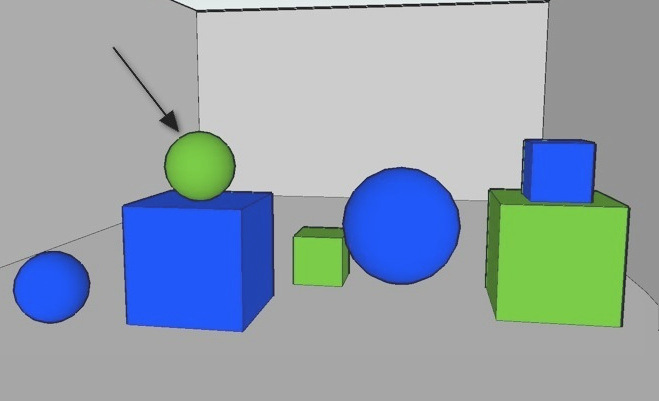
\includegraphics[width=\textwidth]{images/3.jpg}
%\vspace*{1cm}
\caption{Escena 3 del GRE3D7}
\label{GRE3D7-stimulus-3}
\end{minipage}
%\hspace*{-0.35cm}
\begin{minipage}[b]{0.5\linewidth}
\centering
%\begin{figure}[ht]
%\begin{center}
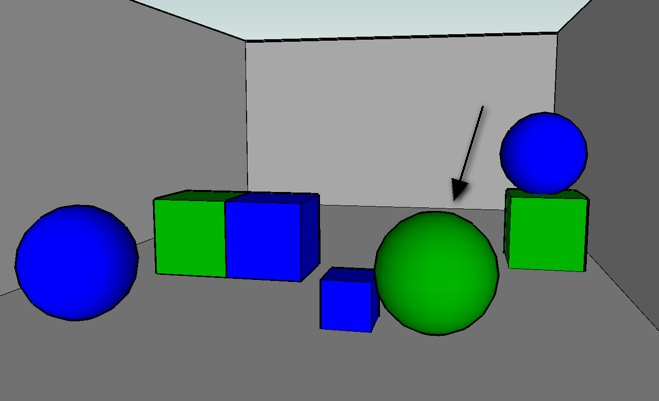
\includegraphics[width=\textwidth]{images/13.jpg}
\caption{Escena 13 del GRE3D7}
\label{GRE3D7-stimulus-13}
\end{minipage}
\end{figure}

\begin{table}[h!]
\begin{center}
\begin{tabular}{|l|c|c|c|c|}
\hline
Palabra &  \puse 					& \puse\ Aprendida & \puse\    							& \puse\  Aprendida \\
        & Modelo \ref{GRE3D7-stimulus-3}   & \ref{GRE3D7-stimulus-3} 				& Modelo \ref{GRE3D7-stimulus-13} 			&  \ref{GRE3D7-stimulus-13}  \\
\hline
esfera & 1.0 & 1.0 & 1.0 & 1.0 \\
cubo & 1.0 & 1.0 & 1.0 & 1.0 \\
verde & 0.978 & 0.993 & 1.0 & 0.9875 \\
peque\~no & 0.257 & 0.346 & 0.0428 & 0.1993 \\
arriba-de & 0.178 & 0.179 & 0 & 0\\ 
azul & 0.15 & 0.124 & 0.064 & 0.1353 \\
grande & 0.107 & 0.03 & 0.307 & 0.7378 \\
izquierda & 0.007 & 0.002 & 0 & 0.0024 \\
arriba & 0.007 & 0 & 0 & 0 \\
derecha & 0 & 0.001 & 0.064 & 0.0005 \\
a-la-izq-de & 0 & 0 & 0 & 0 \\
a-la-der-de & 0 & 0 & 0.064 & 0.1023 \\
debajo-de & 0 & 0 & 0 & 0 \\
\hline
\end{tabular}
\caption{Probabilidades de uso de las palabras del corpus \textit{(GRE3D7) para las Figuras\ref{GRE3D7-stimulus-3} y \ref{GRE3D7-stimulus-13} } 
\label{probability-of-use}}
\end{center}
\end{table}

El aprendizaje se realiza con el kit de herramientas de aprendizaje autom\'atico
WEKA~\cite{Hall:WEK09}, entrenando con todas las escenas menos una (para la que estamos aprendiendo) para todas las escenas del \textit{GRE3D7 y TUNA-corpus}. \\
Ejemplo de xml \ref{archivos-xml-tuna}. Notar que no teniamos las imagenes, armamos algunas necesarias nomas, pero no sabemos la unicaci\'on exacta de los objetos.\\

Un ejemplo de archivo de los que toma WEKA como input es para la propiedad blue de la parte muebles del corpus TUNA es \ref{archivos-arff-blue}. 
No recuerdo si esto lo usamos al final o no...
\ref{probabilidad-GATT} , \ref{algoritmo-GATT} 

Utilizamos regresi\'on lineal para aprender la funci\'on de
\puse\ para cada palabra en la signatura. Para una escena determinada, reemplazamos
las variables de la funci\'on obtenida por los valores de las caracter\'{i}sticas
de la escena que queremos describir.\\

Con regresi\'on lineal podemos aprender caracter\'{i}sticas interesantes
 del dominio. Para empezar, se aprenden hechos conocidos
como que color aparezca en la ER depende en gran medida de si el
target es de ese color, y que no depende de su
poder de discriminaci\'on en el modelo. Por otra parte, vimos que la relaci\'on arriba-de
 se utiliza con m\'as frecuencia que las relaciones horizontales
(izquierda y derecha) lo que confirma un hallazgo previo informado
en~\cite{viet:gene11}. Por \'ultimo, vimos en el
GRE3D7 corpus (que no fue reportado por el trabajo anterior), se utiliza el tama\~no
m\'as frecuentemente de una manera sobreespecificada cuando el
target y el landmark comparten el tama\~no. El tama\~no fue utilizado en ER de manera sobreespecificada en el 49 \% de
las descripciones de escenas en las que el target y el landmark compart\'ian el tama\~no,
y el 25 \% cuando target y el landmark no lo compart\'ian. Esto puede explicarse por la observaci\'on de que si landmark y el target comparten una propiedad, esta propiedad es m\'as relevante.


